\documentclass{beamer}
\usepackage[utf8]{inputenc}
\usepackage[T1]{fontenc}
\usepackage[polish]{babel}

\usepackage{ulem}
\renewcommand<>{\sout}[1]{
    \alt#2{\beameroriginal{\sout}{#1}}{#1}
}
    
\usetheme{Boadilla}

\title{Początki Lispu}
\subtitle{(((Archeologia Cyfrowa)))}
\author{Jakub Grobelny}
\date{19.11.2019}

\begin{document}

%==============================================================================%

\begin{frame}
\titlepage
\end{frame}

\begin{frame}
\frametitle{O czym będzie?}
\tableofcontents
\end{frame}

%==============================================================================%

\section{Do czego był potrzebny taki język?}
\begin{frame}
\frametitle{Narodziny sztucznej inteligencji}
\pause
Lata 50. XX wieku były czasem, gdy sztuczna inteligencja pojawiła się jako 
dziedzina wiedzy.
\pause
\begin{description}
    \item[1950] Alan Turing publikuje ,,\textit{Computing Machinery 
                and Intelligence}''
        \begin{itemize}
            \item \pause 
                \only<-5>{,,\textit{Czy maszyny myślą?}''}
                \only<6-10>{\sout{,,\textit{Czy maszyny myślą?}''}}
            \item \pause 
                \only<-5>{,,\textit{Czy maszyny mogą myśleć?}''}
                \only<6-10>{\sout{,,\textit{Czy maszyny mogą myśleć?}''}}
            \item \pause,,\textit{Czy maszyny mogą działać nieodróżnialnie od ludzi?}''
        \end{itemize} \pause
    \item[1951] Marvin Lee Minsky buduje sieć neuronową 
                SNARC\footnotemark\pause
    \item[1951] Pierwsze programy grające w warcaby (Christopher 
                Strachey) i szachy (Dietrich Prinz)
\end{description}
\only<7-10>{\footnotetext[1]{Stochastic neural analog reinforcement calculator}}
\end{frame}

\begin{frame}
\frametitle{Narodziny sztucznej inteligencji}
\begin{description}
    \item[1955] Allen Newell, Herbert A. Simon i Cliff Shaw
                tworzą program ,,\textit{Logic Theorist}'' \pause
        \begin{itemize}
            \item Program naśladujący ludzkie techniki rozwiązywania 
                  problemów \pause
            \item Program manipulujący \textbf{symbolami} \pause
            \item Udowodnił 38 z pierwszych 52 twierdzeń z ,,\textit{Principia 
                  Mathematica}''\footnotemark \pause \,(niektóre z dowodów były 
                  bardziej eleganckie niż wcześniej istniejące)... \pause
            \item ...i to wszystko zanim określenie ,,sztuczna inteligencja'' w 
            ogóle zostało stworzone.
        \end{itemize}
\end{description}

\only<3-6>{\footnotetext[2]{Autorstwa Alfreda Northa Whiteheada i Bertranda 
                            Russella}}
\end{frame}


\begin{frame}
\frametitle{Narodziny sztucznej inteligencji}

\begin{columns}
\column{0.5\textwidth}

\begin{description}
    \item[1956] Konferencja w Dartmouth. \pause
                \textbf{John McCarthy} przekonuje zebranych do
                używania terminu ,,\textit{sztuczna inteligencja}''.
\end{description}

\column{0.5\textwidth}
\begin{figure}
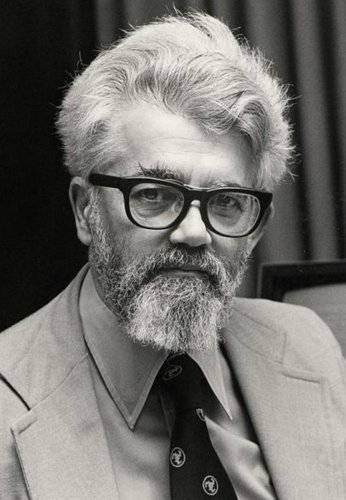
\includegraphics[scale=1.2]{images/mccarthy.jpg}
\caption{John McCarthy}
\end{figure}
\end{columns}
\end{frame}


\begin{frame}
\frametitle{Symbole}
\pause
Okazuje się, że operowanie na \textbf{symbolach} jest istotne przy 
tworzeniu sztucznej inteligencji. \pause

\,\\Ludzkie rozumowanie opiera się na manipulacji symbolami (\textit{physical symbol system hypothesis} -- Allan Newell i Herbert A. Simon)\pause

\,\\System symboli składa się z symboli, składania ich w struktury (wyrażenia) i manipulowania nimi (przetwarzania) w celu tworzenia nowych wyrażeń.

\end{frame}


\begin{frame}
\frametitle{Symbole}

W 1959 roku John McCarthy pisze pracę ,,\textit{Programs with common sense}''.
\pause

\,\\Proponuje w niej stworzenie programu ,,\textit{advice taker}'', który rozwiązywałby problemy poprzez manipulację zdaniami (\textbf{symbole!}).
\pause

\,\\,,\textit{Our ultimate objective is to make programs that 
              learn from their experience as effectively
              as humans do.}''
\end{frame}



\begin{frame}
\frametitle{,,\textit{Programs with common sense}''}
\pause
,,\textit{A class of entities called terms
is defined and a term is an expression. A sequence of expressions is an 
expression. These expressions are represented in the machine by list 
structures}'' -- reprezentacja programów w postaci \textbf{list symboli}
\end{frame}

\begin{frame}
Przykłady:
\pause
    $$at(I, desk)$$
    $$at(desk, home)$$
    $$at(car, home)$$
    $$at(home, county)$$
    $$at(airport, county)$$
\pause
    $$at(x, y), at(y,z) \rightarrow at(x,z)$$
\pause
    $$transitive(at)$$
    $$transitive(u) \rightarrow (u(x,y), u(y,z) \rightarrow u(x,z))$$
\pause
Prawie jak Prolog?
\end{frame}
    


\begin{frame}[fragile]
\frametitle{Zapotrzebowanie na nowe języki}

\begin{columns}
\column{0.6\textwidth}
\textbf{Information Processing Language} \normalsize -- niskopozimowy język 
programowania do manipulowania listami stworzony przez Newella, Shawa i Simona, 
który posłużył do napisania programu
,,\textit{Logic Theorist}''.

\column{0.4\textwidth}
\begin{figure}
\begin{verbatim}
     IPL-V List 
      Structure 
       Example
    Name SYMB LINK
    L1   9-1  100
    100  S4   101
    101  S5   0
    9-1  0    200
    200  A1   201
    201  V1   202
    202  A2   203
    203  V2   0
    
\end{verbatim}
\caption{Kod w IPL}
\end{figure}

\end{columns}

\end{frame}

%==============================================================================%

\section{,,\textit{Recursive Functions of Symbolic Expressions...}''}

\begin{frame}
\end{frame}

%==============================================================================%

\section{Pierwsze implementacje}
\begin{frame}
\end{frame}

%==============================================================================%

\section{Być może coś więcej (Lisp-maszyny, Scheme)}
\begin{frame}
\end{frame}

\end{document}
